% =============================================================
%  Chapitre 5 — DevOps et déploiement
% =============================================================
\chapter{DevOps et déploiement}

\section*{Introduction}
Ce chapitre couvre toute la chaîne de livraison du projet~: de la
conteneurisation Docker à l'orchestration Kubernetes/Helm, en passant
par le pipeline GitHub Actions et la supervision Prometheus/Grafana.

% -----------------------------------------------------------------
\section{Introduction au DevOps et au CI/CD}
% -----------------------------------------------------------------

\textbf{DevOps} désigne un ensemble de pratiques qui rapprochent les
équipes de développement (Dev) et d'exploitation (Ops) pour accélérer
la livraison de logiciels fiables. Les trois axes principaux sont~:

\begin{itemize}
  \item \textbf{L'intégration continue (CI)}~: chaque poussée de code
        déclenche automatiquement la vérification, la compilation et les
        tests du projet~;
  \item \textbf{La livraison continue (CD)}~: le code validé est packagé
        et livré automatiquement sur l'environnement cible~;
  \item \textbf{Le monitoring}~: l'application déployée est surveillée en
        permanence pour détecter anomalies et dégradations de performance.
\end{itemize}

% -----------------------------------------------------------------
\section{Architecture DevOps du projet}
% -----------------------------------------------------------------

\begin{figure}[H]
  \centering
  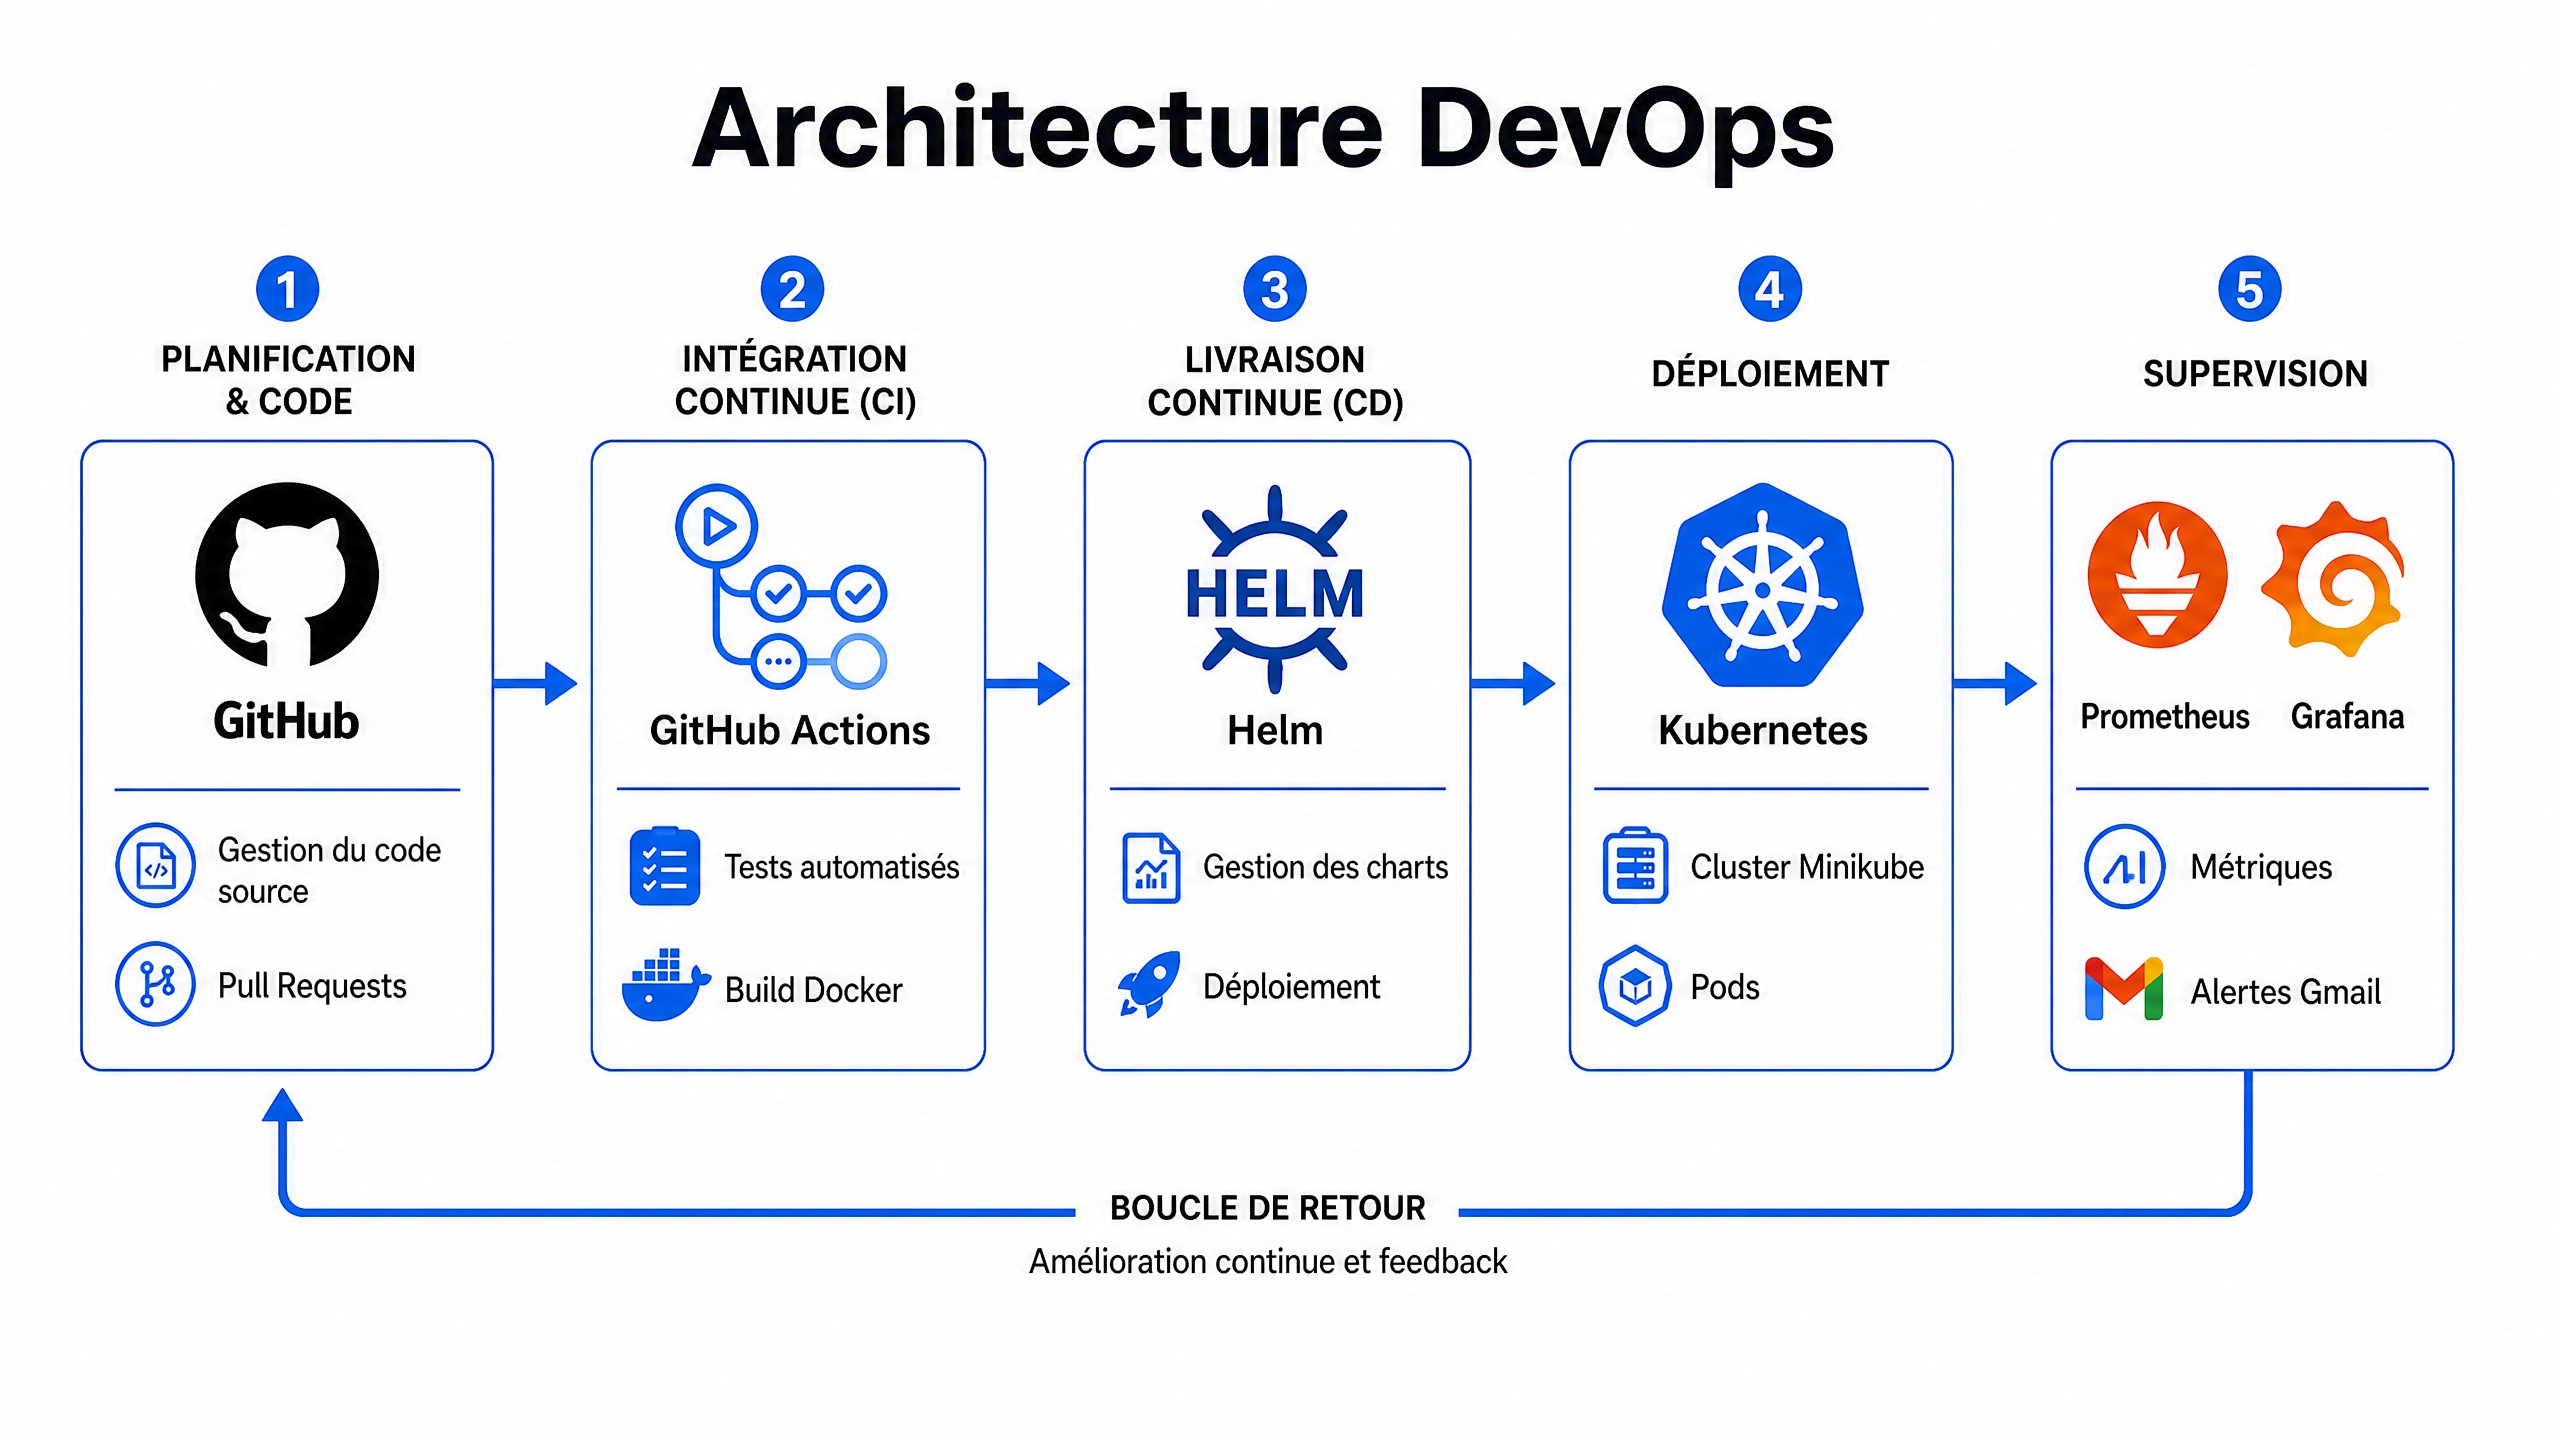
\includegraphics[width=\textwidth]{images/architecture_devops}
  \caption{Architecture DevOps — pipeline CI/CD et infrastructure Kubernetes}
  \label{fig:devops_archi}
\end{figure}

% -----------------------------------------------------------------
\section{Conteneurisation avec Docker}
% -----------------------------------------------------------------

\subsection{Dockerfile du backend}

Le \texttt{Dockerfile} du backend part de l'image \texttt{node:20-alpine},
une base Node.js 20 LTS légère sur Alpine Linux ($\sim$50~Mo). Les
dépendances sont installées avec \texttt{npm ci --only=production} pour
ne pas embarquer les outils de développement. Un argument \texttt{CACHEBUST}
force la re-copie du code source à chaque déploiement. L'application
écoute sur le port 3002 et démarre via \texttt{node src/main/server.js}.

\subsection{Dockerfile du frontend (multi-stage)}

Le \texttt{Dockerfile} du frontend exploite un build \textbf{multi-stage}~:
la première étape utilise \texttt{node:18-alpine} pour compiler l'application
React (\texttt{npm run build}), produisant les fichiers statiques optimisés.
La seconde étape repart d'une image \texttt{nginx:alpine} vierge et y copie
uniquement les fichiers compilés ainsi que la configuration Nginx (reverse proxy).
Cette approche ramène l'image finale de $\sim$900~Mo (avec les dépendances de build)
à $\sim$25~Mo en production.


\subsection{Docker Compose pour le développement}

Le fichier \texttt{docker-compose.yml} orchestre cinq services interdépendants~:
\begin{itemize}
  \item \textbf{mongodb}~: image \texttt{mongo:7} avec volume persistant
        \texttt{mongo-data} et variables d'environnement pour l'initialisation
        de la base~;
  \item \textbf{backend}~: expose les ports 3002 (API REST) et 3003 (WebSocket),
        reçoit la chaîne de connexion MongoDB et le secret JWT via des variables
        d'environnement~;
  \item \textbf{frontend}~: expose le port 3000, dépend du backend~;
  \item \textbf{prometheus}~: image officielle \texttt{prom/prometheus} avec le
        fichier de configuration scrape monté en volume~;
  \item \textbf{grafana}~: image officielle avec datasources et dashboards
        provisionnés automatiquement au démarrage.
\end{itemize}

% -----------------------------------------------------------------
\section{Orchestration avec Kubernetes et Helm}
% -----------------------------------------------------------------

\subsection{Structure des manifestes Kubernetes}

\begin{figure}[H]
  \centering
  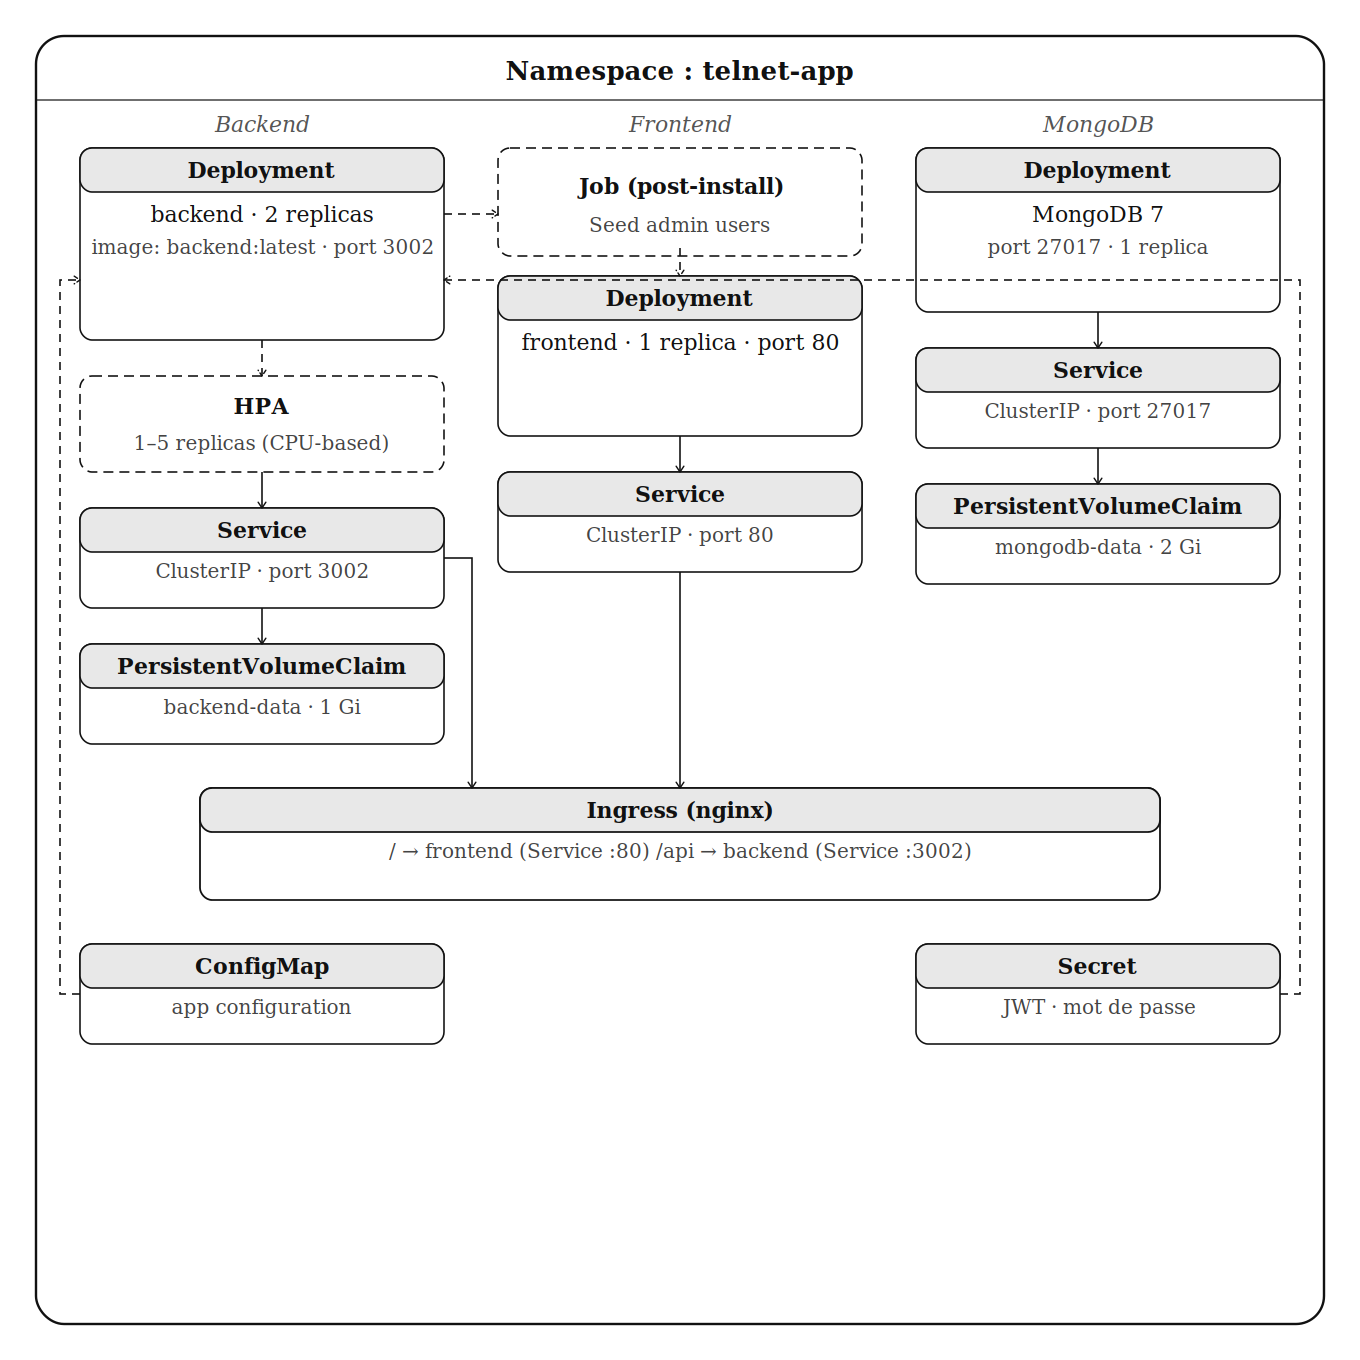
\includegraphics[width=\textwidth]{images/k8s_namespace_v2}
  \caption{Ressources Kubernetes déployées dans le namespace \texttt{telnet-app}}
  \label{fig:k8s_resources}
\end{figure}

\subsection{Chart Helm}

Le chart Helm \texttt{telnet-app} (version~0.3.0) paramétrise l'ensemble
des manifestes Kubernetes. Il comprend 12 templates et expose plus de
40 valeurs configurables dans \texttt{values.yaml}~:

Le fichier \texttt{values.yaml} expose plus de 40 paramètres configurables regroupés
par catégorie~: le nombre de répliques (\texttt{replicaCount}) pour chaque service,
les références d'images Docker (\texttt{image.backend}, \texttt{image.frontend},
\texttt{image.mongodb}), les ports de services, la configuration Ingress
(\texttt{telnet-app.local}), les tailles de volumes persistants (1~Gi pour le backend,
2~Gi pour MongoDB), les paramètres HPA (minReplicas~: 1, maxReplicas~: 5, seuil
CPU~: 70~\%) et les limites de ressources CPU/mémoire pour chaque conteneur.

\subsection{Horizontal Pod Autoscaler}

Le \textbf{HorizontalPodAutoscaler} (version \texttt{autoscaling/v2})
cible le Deployment du backend. Il ajuste automatiquement le nombre de
pods entre 1 et 5 dès que l'utilisation CPU moyenne dépasse 70~\%. Les
seuils (\texttt{minReplicas}, \texttt{maxReplicas} et
\texttt{targetCPUUtilizationPercentage}) sont définis dans
\texttt{values.yaml}, ce qui permet de les modifier sans toucher aux
templates Helm.

\begin{figure}[H]
  \centering
  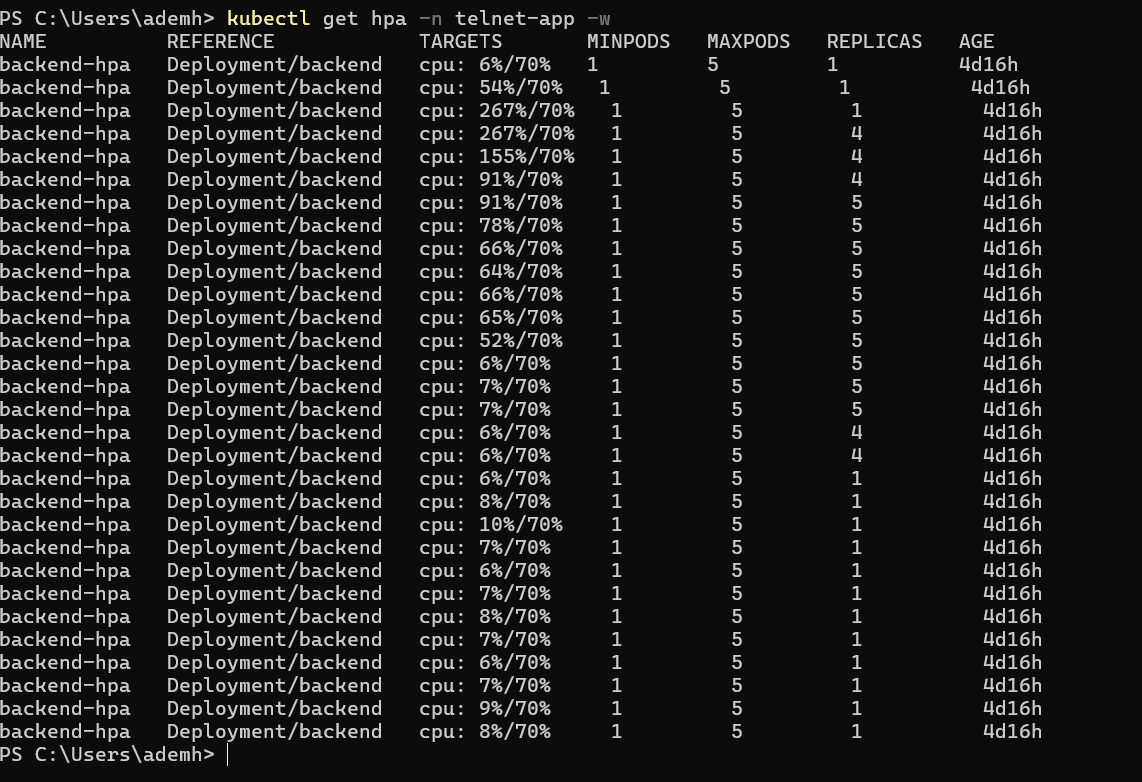
\includegraphics[width=\textwidth]{images/backend replicas after load test}
  \caption{Montée en charge HPA --- répliques backend passant de 1 à 5 sous stress CPU (267\,\%/70\,\%)}
  \label{fig:hpa_scaling}
\end{figure}

\subsection{Stratégie de déploiement Rolling Update}

Kubernetes utilise par défaut une stratégie de \textbf{rolling update}~:
les nouveaux pods démarrent progressivement pendant que les anciens
restent actifs, ce qui évite toute interruption de service.

Le Deployment backend est configuré avec \texttt{maxUnavailable~: 0} et
\texttt{maxSurge~: 1}. Concrètement, aucun pod n'est supprimé tant que
le nouveau n'est pas prêt, et un pod supplémentaire est autorisé pendant
la transition. Résultat~: les mises à jour se font en \textit{zero downtime}.

% -----------------------------------------------------------------
\section{Pipeline GitHub Actions}
% -----------------------------------------------------------------

\subsection{Vue d'ensemble du workflow}

Le workflow \texttt{ci-cd.yaml} se déclenche sur tout push vers \texttt{main} ou
\texttt{develop} et sur les pull requests vers \texttt{main}. Un mécanisme de
\texttt{concurrency} annule les exécutions précédentes de la même branche pour
éviter les déploiements en parallèle. Le pipeline comprend trois jobs~:

\begin{itemize}
  \item \textbf{ci-backend} (runner Ubuntu)~: installation des dépendances
        (\texttt{npm ci}), audit de sécurité (\texttt{npm audit --audit-level=critical})
        et exécution des tests unitaires~;
  \item \textbf{ci-frontend} (runner Ubuntu)~: mêmes étapes plus un build de
        production React (\texttt{npm run build})~;
  \item \textbf{deploy} (runner auto-hébergé, branche \texttt{main} uniquement)~:
        démarrage de Minikube si nécessaire, construction des images Docker dans le
        daemon Minikube, déploiement via \texttt{helm upgrade --install --atomic} avec
        injection des secrets depuis les variables GitHub Actions, puis attente du
        rollout avec \texttt{kubectl rollout status}.
\end{itemize}

À l'issue du déploiement, un résumé est automatiquement généré dans
l'interface GitHub Actions via \texttt{\$GITHUB\_STEP\_SUMMARY}~: il
récapitule le commit, la branche, l'heure de déploiement et l'état
des pods dans les namespaces \texttt{telnet-app} et \texttt{monitoring}.

\subsection{Configuration du runner auto-hébergé}

Le job \texttt{deploy} s'exécute sur un runner \textbf{auto-hébergé}
(\textit{self-hosted}) installé directement sur la machine Windows locale
hébergeant Minikube. Cette configuration est nécessaire car~:
\begin{itemize}
  \item L'accès au cluster Minikube est local et non exposé sur Internet~;
  \item Les images Docker doivent être construites dans le daemon Docker
        de Minikube (sans registry externe)~;
  \item Les secrets d'infrastructure restent dans l'environnement local.
\end{itemize}

Le runner est enregistré sur GitHub via~:
L'enregistrement du runner s'effectue en deux commandes~: \texttt{config.cmd}
reçoit l'URL du dépôt, un token d'authentification éphémère et les labels
(\texttt{self-hosted}, \texttt{windows}, \texttt{minikube}) qui permettent au
job \texttt{deploy} de le cibler. La commande \texttt{run.cmd} démarre ensuite
le runner en écoute permanente des jobs GitHub Actions.

% -----------------------------------------------------------------
\section{Supervision avec Prometheus et Grafana}
% -----------------------------------------------------------------

\subsection{Métriques Prometheus}

Quatre métriques personnalisées sont exposées sur \texttt{/metrics}~:

\begin{table}[H]
  \centering
  \caption{Métriques Prometheus de Telnet Test Manager}
  \label{tab:prometheus_metrics}
  \begin{tabularx}{\textwidth}{|L{6.2cm}|L{2.3cm}|X|}
    \hline
    \textbf{Métrique} & \textbf{Type} & \textbf{Description} \\
    \hline
    {\small\texttt{http\_requests\_total}} & Counter &
      Nombre total de requêtes HTTP par méthode, route et code de statut \\
    \hline
    {\small\texttt{http\_request\_duration\_seconds}} & Histogram &
      Distribution des temps de réponse par route (buckets~: 10\,ms à 5\,s) \\
    \hline
    {\small\texttt{telnet\_tests\_launched\_total}} & Counter &
      Nombre total de tests Telnet lancés \\
    \hline
    {\small\texttt{websocket\_active\_connections}} & Gauge &
      Nombre de connexions WebSocket actives en temps réel \\
    \hline
  \end{tabularx}
\end{table}

Le module \texttt{prometheusMetrics.js} active d'abord la collecte des métriques
par défaut de la VM Node.js via \texttt{collectDefaultMetrics} (CPU, mémoire, heap,
event loop). Il définit ensuite quatre métriques personnalisées~: un \texttt{Counter}
\texttt{http\_requests\_total} labellisé par méthode, route et code HTTP~; un
\texttt{Histogram} \texttt{http\_request\_duration\_seconds} avec 8 buckets de
10~ms à 5~s~; un \texttt{Counter} \texttt{telnet\_tests\_launched\_total} incrémenté
à chaque appel à \texttt{/run-test}~; et une \texttt{Gauge}
\texttt{websocket\_active\_connections} mise à jour à chaque connexion ou
déconnexion WebSocket.

\subsection{Tableau de bord Grafana}

Le tableau de bord \textbf{«~Telnet Test Manager~--- Monitoring~»} est
provisionné automatiquement au démarrage de Grafana via un fichier JSON.
Il comprend dix panneaux~:

\begin{table}[H]
  \centering
  \caption{Panneaux du tableau de bord Grafana}
  \label{tab:grafana_panels}
  \begin{tabularx}{\textwidth}{|L{4.5cm}|L{2.5cm}|X|}
    \hline
    \textbf{Panneau} & \textbf{Type} & \textbf{Requête PromQL} \\
    \hline
    Backend UP/DOWN & Stat &
      \texttt{up\{job="backend"\}} \\
    \hline
    Tests Telnet lancés & Stat &
      \texttt{telnet\_tests\_launched\_total} \\
    \hline
    Requêtes HTTP totales & Stat &
      \texttt{sum(http\_requests\_total)} \\
    \hline
    RAM Backend (Mo) & Stat &
      {\small\texttt{process\_resident\_memory\_bytes / 1024\^{}2}} \\
    \hline
    Taux de requêtes par route & Séries temp. &
      \texttt{rate(http\_requests\_total[1m])} \\
    \hline
    Durée p95 des requêtes & Séries temp. &
      {\small\texttt{histogram\_quantile(0.95,}}\newline
      {\small\texttt{rate(http\_request\_duration\_}}\newline
      {\small\texttt{seconds\_bucket[1m]))}} \\
    \hline
    Connexions WebSocket & Séries temp. &
      \texttt{websocket\_active\_connections} \\
    \hline
    CPU Backend (\%) & Jauge &
      {\small\texttt{rate(process\_cpu\_seconds\_total[1m])}}\newline
      {\small\texttt{* 100}} \\
    \hline
    Requêtes par code statut & Barres &
      {\small\texttt{sum by (status)}}\newline
      {\small\texttt{(http\_requests\_total)}} \\
    \hline
    Top 5 routes par latence & Tableau &
      {\small\texttt{avg by (route)}}\newline
      {\small\texttt{(http\_request\_duration\_seconds)}} \\
    \hline
  \end{tabularx}
\end{table}

Une règle d'alerte \textbf{Backend CPU High} est configurée~: lorsque
l'utilisation CPU dépasse le seuil de 70\,\%, Grafana envoie automatiquement
une notification par e-mail avec le niveau de sévérité \texttt{CRITICAL}.

\begin{figure}[H]
  \centering
  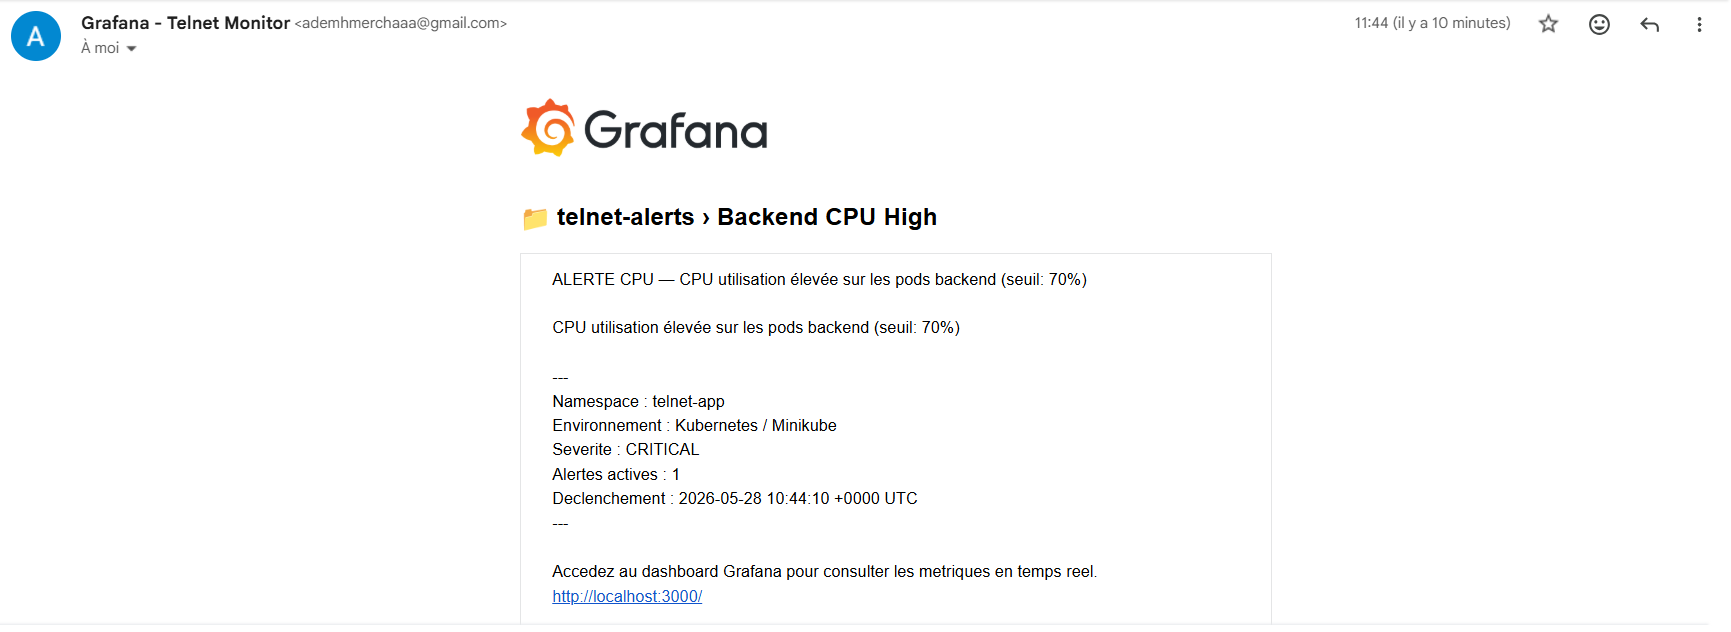
\includegraphics[width=0.85\textwidth]{images/grafana alert}
  \caption{Alerte e-mail Grafana --- déclenchement automatique sur dépassement CPU (seuil~: 70\,\%)}
  \label{fig:grafana_alert}
\end{figure}

% -----------------------------------------------------------------
\section{Infrastructure as Code}
% -----------------------------------------------------------------

L'\textbf{Infrastructure as Code} (IaC) consiste à gérer l'infrastructure
via des fichiers de configuration versionnés, comme on le ferait pour
du code applicatif. Ce projet l'applique à trois niveaux.

\subsection{Helm Charts}

Le chart Helm \texttt{telnet-app} (version~0.3.0) est la source unique
de vérité pour tout le déploiement Kubernetes. Il comprend 12 templates
paramétrables et expose plus de 40 valeurs configurables dans
\texttt{values.yaml}. Toute modification d'infrastructure (ressources,
répliques, secrets) passe par ce fichier versionné dans Git.

\begin{figure}[H]
  \centering
  \begin{lstlisting}[basicstyle=\ttfamily\small, frame=single, backgroundcolor=\color{gray!6}]
helm/telnet-app/
|-- Chart.yaml
|-- values.yaml
`-- templates/
    |-- backend-deployment.yaml
    |-- backend-service.yaml
    |-- backend-hpa.yaml
    |-- backend-pvc.yaml
    |-- frontend-deployment.yaml
    |-- frontend-service.yaml
    |-- mongodb-deployment.yaml
    |-- mongodb-service.yaml
    |-- mongodb-pvc.yaml
    |-- mongodb-initdb-configmap.yaml
    |-- configmap.yaml
    |-- secret.yaml
    |-- ingress.yaml
    `-- seed-job.yaml
  \end{lstlisting}
  \caption{Structure du chart Helm \texttt{telnet-app} --- 14 templates paramétrables}
  \label{fig:helm_structure}
\end{figure}

\subsection{Manifestes Kubernetes}

Chaque ressource Kubernetes est générée depuis le chart Helm~:
Deployments, Services, HPA, Ingress, PersistentVolumeClaims, ConfigMap
et Secrets. Les secrets applicatifs (mot de passe MongoDB, JWT secret,
SMTP) sont injectés via des variables de pipeline GitHub Actions
(\texttt{secrets.MONGO\_PASSWORD}, etc.) et ne sont jamais commités
dans le dépôt.

\begin{figure}[H]
  \centering
  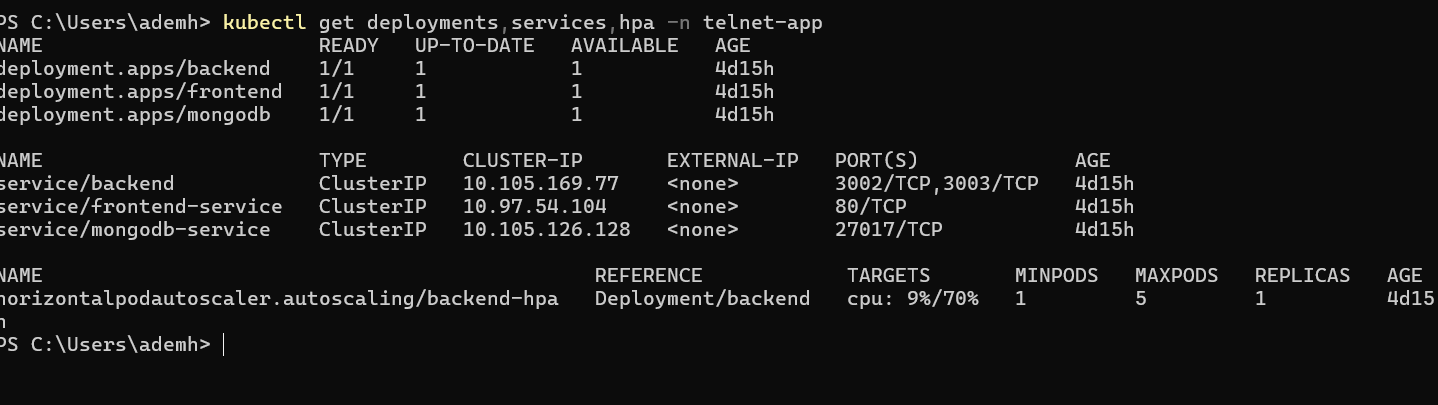
\includegraphics[width=\textwidth]{images/kubernetes deployements manifests}
  \caption{Ressources Kubernetes déployées dans le namespace \texttt{telnet-app}}
  \label{fig:kubectl_telnet}
\end{figure}

\begin{figure}[H]
  \centering
  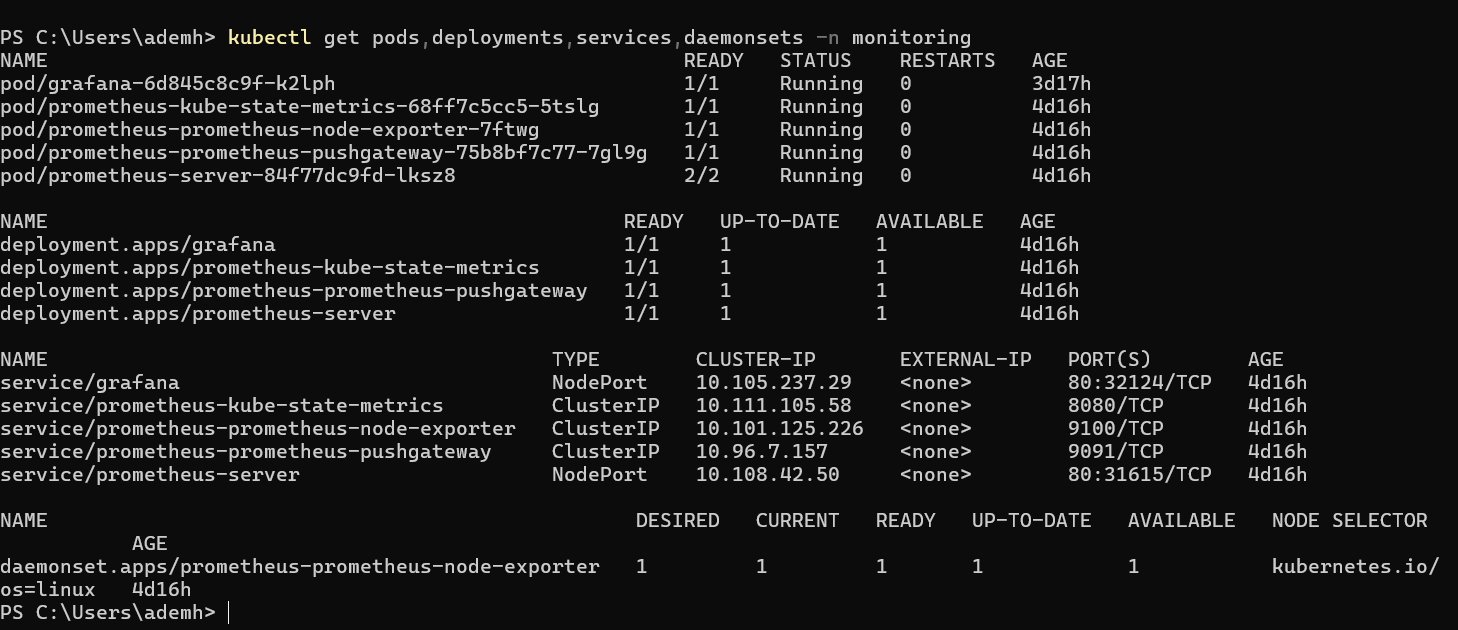
\includegraphics[width=\textwidth]{images/gafana_promethus manifeests}
  \caption{Ressources Kubernetes déployées dans le namespace \texttt{monitoring} (Prometheus et Grafana)}
  \label{fig:kubectl_monitoring}
\end{figure}

\subsection{Automatisation}

L'ensemble du cycle de vie de l'infrastructure est automatisé~:
\begin{itemize}
  \item \textbf{Provisioning}~: \texttt{helm upgrade --install} crée
        ou met à jour toutes les ressources de manière idempotente~;
  \item \textbf{Seeding}~: un Job Kubernetes post-install initialise
        les utilisateurs de démonstration en base MongoDB~;
  \item \textbf{Monitoring}~: Prometheus et Grafana sont déployés via
        leurs propres charts Helm avec dashboards et alertes provisionnés
        en code (\texttt{grafana-values.yaml})~;
  \item \textbf{Rollback}~: \texttt{helm rollback telnet-app}
        restaure en un seul appel la version précédente.
\end{itemize}

\begin{figure}[H]
  \centering
  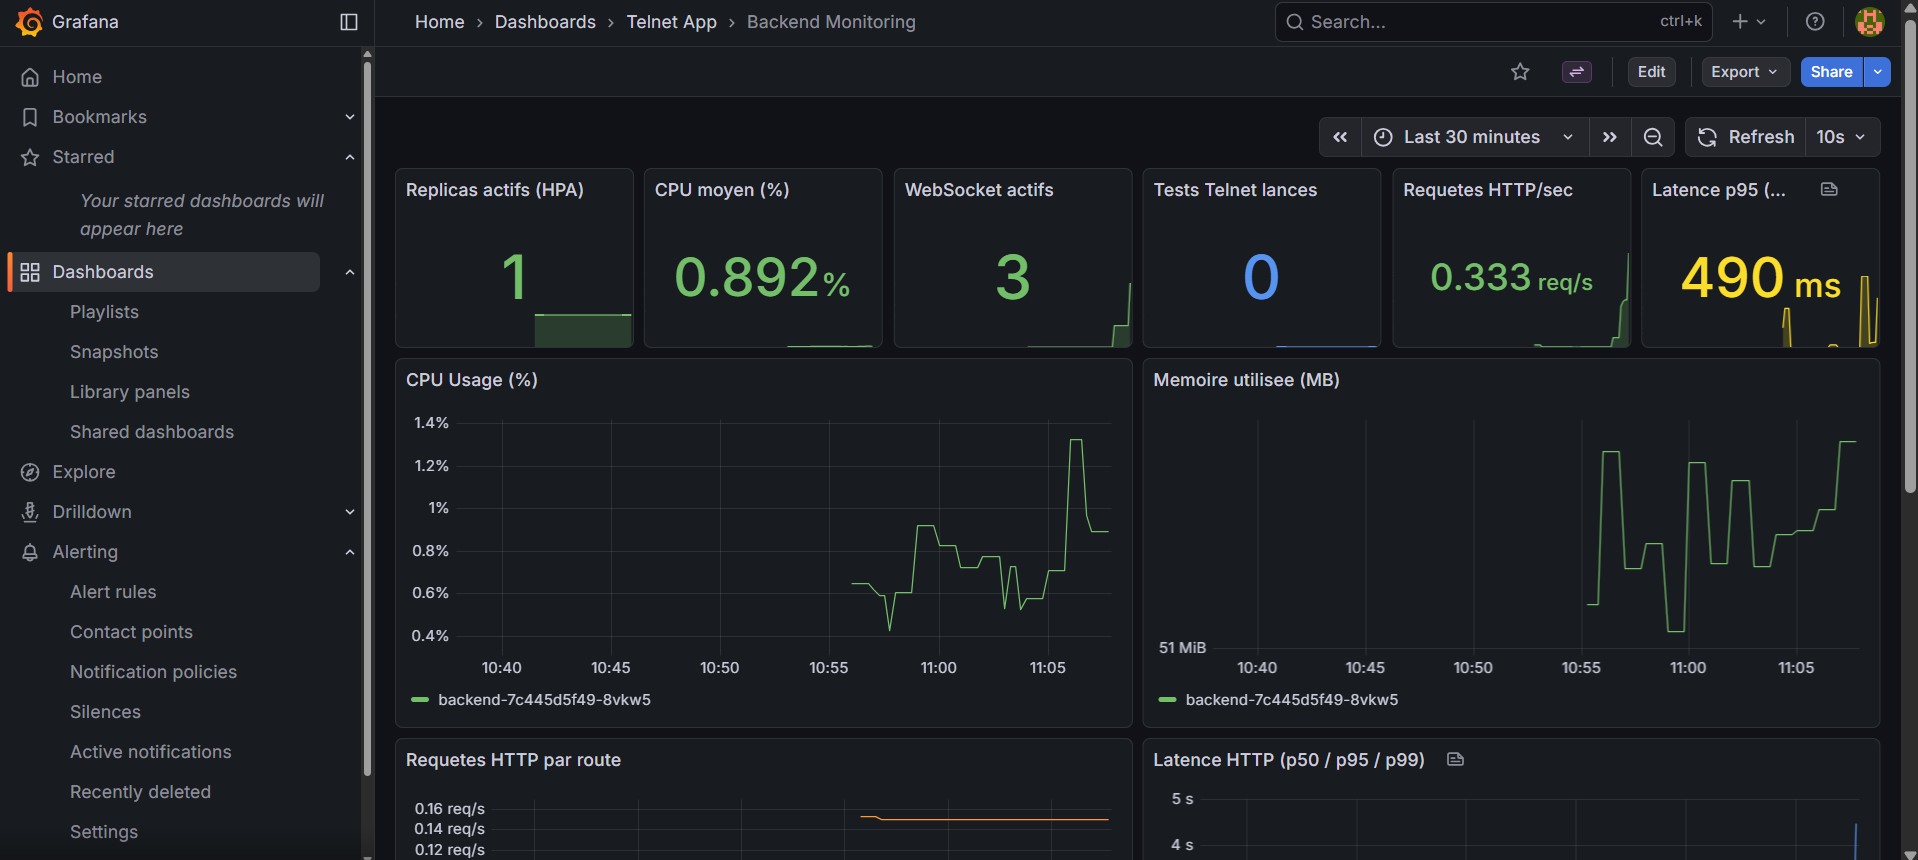
\includegraphics[width=\textwidth]{images/capture grafana metrics}
  \caption{Tableau de bord Grafana --- Telnet Test Manager}
  \label{fig:screen_grafana}
\end{figure}

\begin{figure}[H]
  \centering
  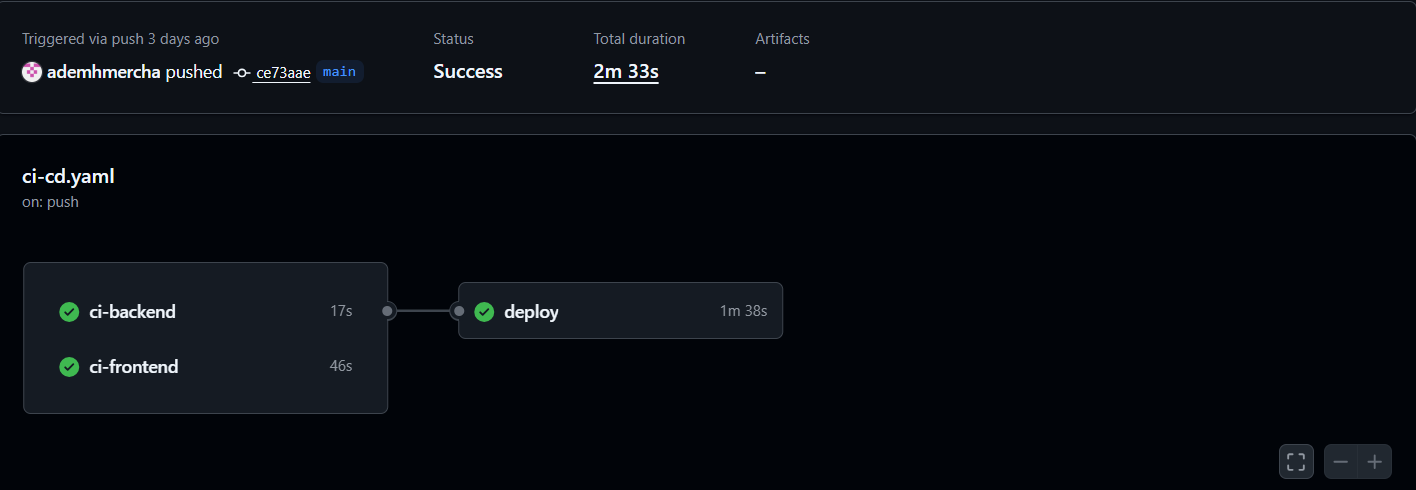
\includegraphics[width=\textwidth]{images/captre du pipeline}
  \caption{Capture d'écran~: exécution du pipeline CI/CD sur GitHub Actions}
  \label{fig:screen_pipeline}
\end{figure}

% -----------------------------------------------------------------
\section{Tests et validation}
% -----------------------------------------------------------------

\subsection{Stratégie de tests}

La qualité du projet est validée selon la \textbf{pyramide de tests}
classique~: un grand nombre de tests unitaires rapides, des tests
d'intégration couvrant l'API REST, et des tests fonctionnels manuels.

\begin{figure}[H]
  \centering
  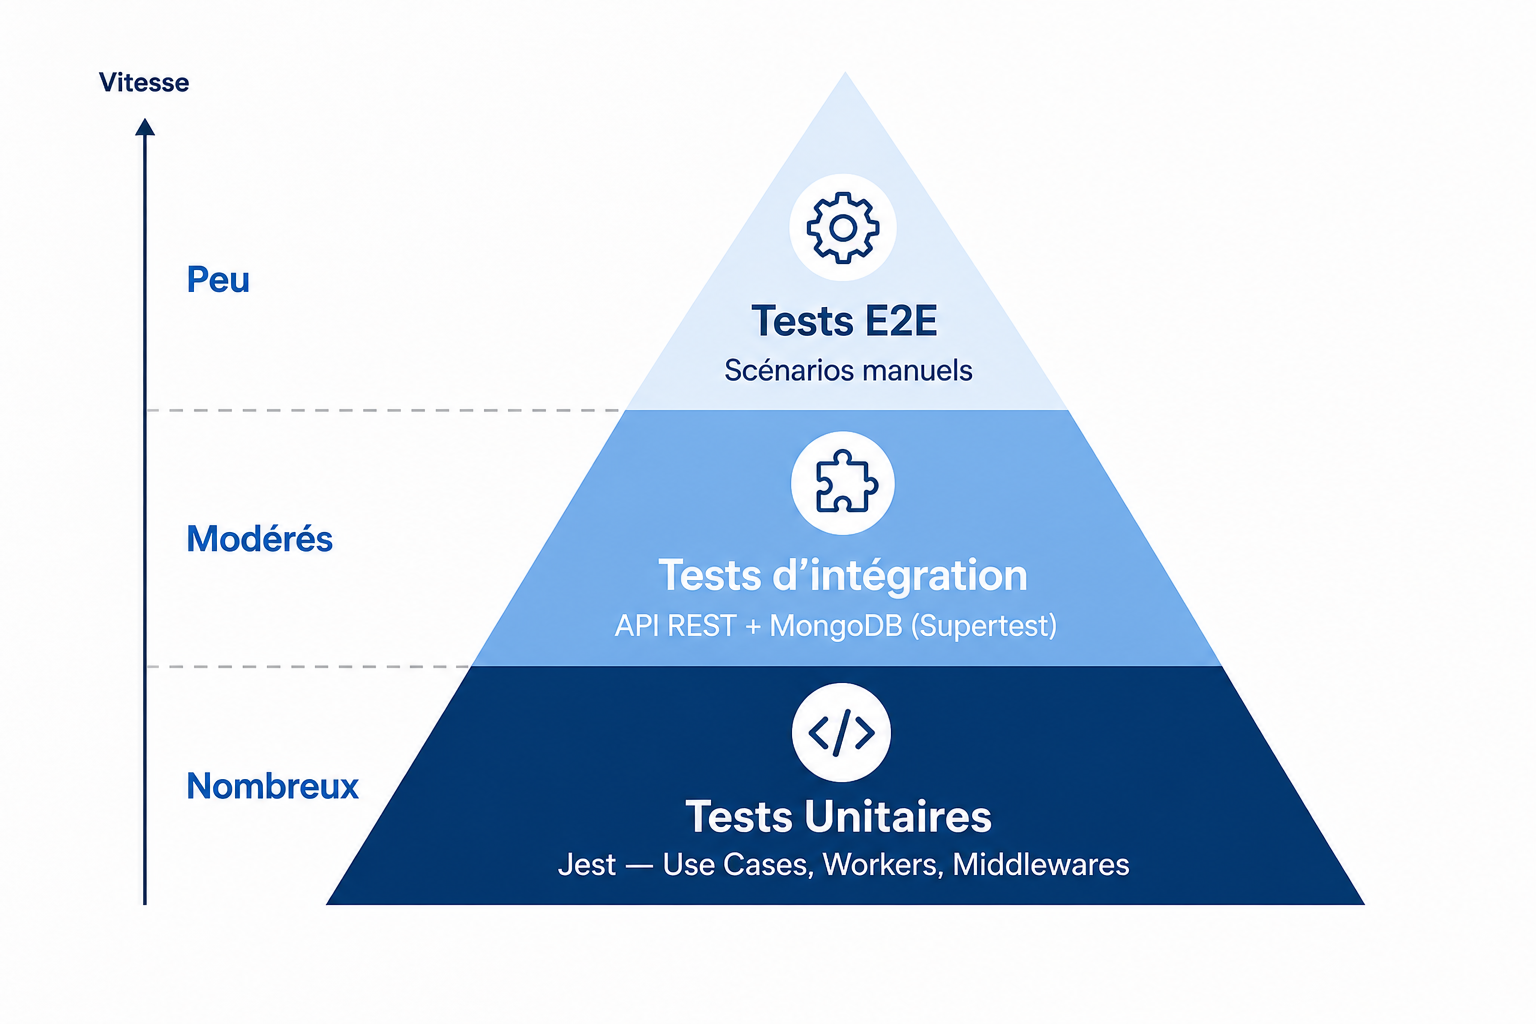
\includegraphics[width=0.75\textwidth]{images/pyramide_tests}
  \caption{Pyramide de tests adoptée pour Telnet Test Manager}
  \label{fig:test_pyramid}
\end{figure}

\subsection{Tests unitaires (Jest)}

Les tests unitaires couvrent les Use Cases et les modules critiques.
Les dépendances externes (MongoDB, réseau Telnet) sont mockées.

Deux cas de test couvrent le Use Case d'authentification~: le premier vérifie qu'un
appel avec des identifiants corrects retourne bien un objet contenant un champ
\texttt{token} (JWT signé)~; le second vérifie que l'exécution est rejetée avec
l'erreur \texttt{Compte inactif} lorsque le champ \texttt{statut} de l'utilisateur
vaut \texttt{inactif}. Le dépôt MongoDB est entièrement mocké via \texttt{jest.fn()},
garantissant l'isolation du test vis-à-vis de la base de données.

Les tests d'intégration utilisent \textbf{Supertest} avec une base
MongoDB de test isolée. Ils couvrent l'authentification, les endpoints
CRUD et la limitation de débit (rate limiting).

\begin{figure}[H]
  \centering
  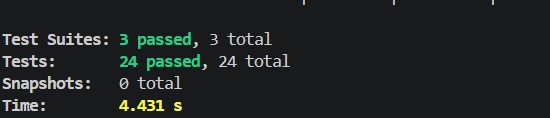
\includegraphics[width=0.7\textwidth]{images/jest_results}
  \caption{Résultats des tests Jest --- 24 tests passés sur 24 (3 suites)}
  \label{fig:screen_jest}
\end{figure}

\subsection{Tests fonctionnels (scénarios E2E)}

\begin{table}[H]
  \centering
  \caption{Scénarios de tests fonctionnels --- résultats}
  \label{tab:e2e_tests}
  \begin{tabularx}{\textwidth}{|C{1.2cm}|X|L{3.8cm}|L{2.2cm}|}
    \hline
    \textbf{ID} & \textbf{Scénario} & \textbf{Précondition} & \textbf{Résultat} \\
    \hline
    ST01 & Connexion identifiants valides   & Utilisateur actif en BD   & \textcolor{vertCode}{\textbf{PASS}} \\
    \hline
    ST02 & Connexion mot de passe erroné    & ---                       & \textcolor{vertCode}{\textbf{PASS}} \\
    \hline
    ST03 & Accès route protégée sans JWT    & ---                       & \textcolor{vertCode}{\textbf{PASS}} \\
    \hline
    ST04 & Création d'un Poste (CRUD)       & Rôle ingénieur            & \textcolor{vertCode}{\textbf{PASS}} \\
    \hline
    ST05 & Création Slot avec adresse IP    & Poste + Produit existants & \textcolor{vertCode}{\textbf{PASS}} \\
    \hline
    ST06 & Exécution test \texttt{single}   & Slot actif                & \textcolor{vertCode}{\textbf{PASS}} \\
    \hline
    ST07 & Exécution test séquence 3 étapes & Slot actif                & \textcolor{vertCode}{\textbf{PASS}} \\
    \hline
    ST08 & Résultats temps réel (WebSocket) & Test en cours             & \textcolor{vertCode}{\textbf{PASS}} \\
    \hline
    ST09 & Arrêt d'un test en cours         & Test PENDING              & \textcolor{vertCode}{\textbf{PASS}} \\
    \hline
    ST10 & Tests multi-slots (3 parallèles) & 3 slots configurés        & \textcolor{vertCode}{\textbf{PASS}} \\
    \hline
    ST11 & Génération d'un rapport          & Tests historisés           & \textcolor{vertCode}{\textbf{PASS}} \\
    \hline
    ST12 & Consultation journal d'audit     & Rôle admin                & \textcolor{vertCode}{\textbf{PASS}} \\
    \hline
    ST13 & Changement de langue (FR~$\to$~EN) & ---                     & \textcolor{vertCode}{\textbf{PASS}} \\
    \hline
    ST14 & Accès technicien à route admin   & JWT technicien            & \textcolor{vertCode}{\textbf{PASS}} \\
    \hline
  \end{tabularx}
\end{table}

\subsection{Résultats du pipeline CI/CD}

\begin{table}[H]
  \centering
  \caption{Résultats du pipeline GitHub Actions}
  \label{tab:cicd_results}
  \begin{tabularx}{\textwidth}{|L{2.5cm}|X|L{2.8cm}|L{2.5cm}|}
    \hline
    \textbf{Job} & \textbf{Étapes clés} & \textbf{Durée} & \textbf{Statut} \\
    \hline
    ci-backend  & npm ci + audit + tests        & 17\,s         & \textcolor{vertCode}{\textbf{Success}} \\
    \hline
    ci-frontend & npm ci + audit + build        & 46\,s         & \textcolor{vertCode}{\textbf{Success}} \\
    \hline
    deploy      & Build Docker + Helm + rollout & 1\,min\,38\,s & \textcolor{vertCode}{\textbf{Success}} \\
    \hline
    \textbf{Total} & --- & \textbf{2\,min\,33\,s} & \textcolor{vertCode}{\textbf{Success}} \\
    \hline
  \end{tabularx}
\end{table}

\subsection{Tableau de synthèse de validation}

\begin{table}[H]
  \centering
  \caption{Synthèse de la validation par rapport aux besoins}
  \label{tab:synthese_validation}
  \begin{tabularx}{\textwidth}{|C{1.2cm}|X|L{3.8cm}|L{2.2cm}|}
    \hline
    \textbf{BF} & \textbf{Besoin} & \textbf{Méthode de test} & \textbf{Statut} \\
    \hline
    BF-01 & Authentification JWT           & Tests unit. + intégration  & \textcolor{vertCode}{Validé} \\
    \hline
    BF-02 & Gestion des équipements CRUD   & Tests intégration          & \textcolor{vertCode}{Validé} \\
    \hline
    BF-03 & Bibliothèque de commandes      & Tests intégration          & \textcolor{vertCode}{Validé} \\
    \hline
    BF-04 & Tests multi-slots parallèles   & Tests fonctionnels         & \textcolor{vertCode}{Validé} \\
    \hline
    BF-05 & Résultats temps réel (WS)      & Tests fonctionnels         & \textcolor{vertCode}{Validé} \\
    \hline
    BF-06 & Exécution test Telnet          & Tests unit. + fonctionnels & \textcolor{vertCode}{Validé} \\
    \hline
    BF-07 & Génération de rapports         & Tests fonctionnels         & \textcolor{vertCode}{Validé} \\
    \hline
    BF-08 & Administration (RBAC)          & Tests unit. + intégration  & \textcolor{vertCode}{Validé} \\
    \hline
    ---   & Pipeline CI/CD                 & Exécution GitHub Actions   & \textcolor{vertCode}{Validé} \\
    \hline
    ---   & Déploiement Kubernetes         & \texttt{kubectl rollout}   & \textcolor{vertCode}{Validé} \\
    \hline
    ---   & Supervision Prometheus/Grafana & Consultation dashboard     & \textcolor{vertCode}{Validé} \\
    \hline
  \end{tabularx}
\end{table}

\section*{Conclusion}

Ce chapitre a détaillé l'infrastructure DevOps complète et la validation
du projet Telnet Test Manager. La conteneurisation Docker, l'orchestration
Kubernetes/Helm avec autoscaling HPA, le pipeline GitHub Actions en trois
jobs et la supervision Prometheus/Grafana constituent un système de
déploiement mature et automatisé. Le taux de réussite de 100\,\% sur les
14~scénarios fonctionnels testés et la validation de l'ensemble des
besoins fonctionnels confirment la qualité de la réalisation.
